\newcommand{\NbasesV}{\textit{N}}
\newcommand{\Nbases}{6}
\newcommand{\Nml}{6}
\newcommand{\NmlT}{5}
\newcommand{\NmlA}{2}
\newcommand{\Ncb}{4}
\newcommand{\MML}{método multirrótulo}
\newcommand{\MMLs}{métodos multirrótulo}
\newcommand{\MRLM}{Recursive Dependent Binary Relevance}
\newcommand{\MRLMa}{RDBR}

\chapter{Introdução}
Segundo \cite{rezende2003sistemas} Aprendizado de Máquina é uma área de Inteligência Artificial
cujo objetivo é o desenvolvimento de técnicas computacionais
sobre o aprendizado bem como a construção de sistemas capazes de adquirir
conhecimento de forma automática. Essa área tem atraido a atenção de muitos 
pesquisadores em diversas especialidades. Dentro dessa área, encontra-se a subárea Aprendizado Supervisionado.
Em Aprendizado Supervisionado, um problema de classificação é a tarefa de encontrar
uma técnica capaz de predizer a classe ou as classes que uma instância de
um objeto em específico pertence \cite{rezende2003sistemas}.
Para completar essa tarefa, a técnica deve usar exemplos de treino cujas as classes
são conhecidas que lhe são dispostas. Uma instância é um objeto do mundo real descrito
por um vetor de valores numéricos ou nominais e por um conjunto de rótulos.
Na literatura, as classes também são chamadas de rótulos (REZENDE, 2003, p. 91)
e quando as instâncias só podem assumir um único rótulo, o problema é chamado de classificação unirrótulo,
do contrário, é chamado de problema de classificação multirrótulo (BORGES, 2012).

Problemas de classificação multirrótulo estão presentes em diversas áreas, trabalhos relevantes podem
ser encontrados em áreas como a bioinfomática, diagnóstico médico, classificação de imagens e principalmente
categorização de textos (CARVALHO, 2009, p. 2). A classificação multirrótulo é inevitavelmente
mais complexa que a unirrótulo. Para solucioná-la,  o método multirrótulo mais conhecido é um método simples chamado de
Relevância Binária (BR – Binary Relevance) (READ, 2011, p. 2). 
Há muitas críticas sobre o método, sendo a maior delas a incapacidade do método de reconhecer correlação entre os rótulos (READ, 2011, p. 2).
Com o intuito de alcançar melhores resultados que o BR, alguns autores o aprimoraram ou elaboraram novos tipos de métodos
de tal forma que divergem na forma como resolvem o problema (READ, 2011). 
Por exemplo, existem métodos que transformam o problema multirrótulo em
diversos problemas unirrótulo, como é o caso do BR, e outros métodos que são classificadores especiais, capazes de classificar diretamente sobre os problemas multirrótulo, sem necessidade de transformação, como é o caso do Multi-Label C4.5 (MADJAROV et al., 2012, p. 5). 

Com tantos métodos novos, alguns deles apresentados por Carvalho (2009)
e por Read(2011) é necessário realizar comparações e testes de qualidade.
É certo que já existem análises e comparações entre os métodos,
no entanto há necessidade de avaliar os métodos de forma mais formal
e reforçar as conclusões alcançadas pelos autores dos métodos além de elaborar
uma forma eficiente de comparar tipos diferentes de métodos multirrótulos (DRUMMOND, 2008).

\section{Motivações}
% A análise dos métodos multirrótulo traz os seguintes benefícios:
O melhor entendimento do funcionamento dos métodos multirrótulo permite:
\begin{itemize}
 \item descobrir atributos destes que se alterados, aproveitados
 e/ou combinados podem acarretar na criação de novos métodos e/ou na melhora dos existentes.
 \item prever, com uma certa taxa de erro, seus desempenhos, o que facilita o uso mais inteligente dos métodos
 sem precisar utilizar muito esforço computacional devido a testes.
 \item reforçar ou contrariar as conclusões já estabelecidas dos métodos, uma vez que a maioria delas são 
 baseadas em testes experimentais.
\end{itemize}

\section{Objetivos}
O objetivo geral deste trabalho é analisar e comparar métodos multirrótulos distintos e 
desenvolver um novo algoritmo de classificação multirrótulo.
Mais formalmente, a análise deve implicar em conclusões matemáticas ou estatísticas sobre o desempenho dos métodos multirrótulo.
O Objetivo geral pode ser detalhado nos seguintes objetivos específicos:
\begin{itemize}
 \item Comparação estatística e análise crítica dos métodos multirrótulos;
 \item Elaboração de um algoritmo de um novo método multirrótulo.
 \item Implementação dos métodos multirrótulos em uma biblioteca que integra técnicas de reconhecimento de padrões.
\end{itemize}


% \section{Contribuições}
\section{Estrutura do Trabalho}
O restante do trabalho está organizado da seguinte forma:
\begin{itemize}
 \item O capítulo 2 apresenta os principais conceitos da classificação multirrótulo, bem como
 os métodos usados para avaliação de desempenho de classificadores multirrótulo.
 \item O capítulo 3 apresenta a definição de diferentes métodos de classificação multirrótulo usados neste trabalho,
 bem como suas complexidades algorítma.
 \item O capítulo 4 apresenta a definição de um novo método de classificação multirrótulo proposto neste trabalho.
 \item O capítulo 5 começa apresentando as configurações experimentais escolhidos para realização de testes e termina
 apresentando os resultados e a sua análise detalhada.
 \item No capítulo 6 são apresentados as conclusões finais sobre o desempenho dos métodos e sobre a análise do capítulo anterior.
\end{itemize}


\chapter{Classificação multirrótulo}

Problemas de classificação estão situadas na área de aprendizado supervisionado, que por sua vez é uma 
subárea da mineração de dados. Para \cite{dunham2003introductory} a mineração de dados é definido como a descoberta
de informações escondidas em um conjunto de dados. Ela surgiu diante do grande crescimento de dados armazenados
em arquivos de computadores e do desejo dos usuários desses dados em obter informações mais detalhadas do que simplesmente
os próprios dado em si. A mineração de dados tem por objetivo satisfazer o desejo desses usuários ao desenvolver técnicas
capazes de explicitar informações valiosas, antes escondidas ao usuários diante de uma alta quantidade de dados.
Uma de suas subáreas é a aprendizado supervisionado. Nela, segundo \cite{mohri2012foundations},
os dados pelos quais deve-se extrair as informações são associados a uma variável especial cujo valor
é conhecido e a técnica deve predizer os rótulos
corretamente para novos dados cujo valor da variável especial associada a elas é desconhecido.

Normalmente, em aprendizado supervisionado os dados são objetos de um domínio específico e cada um dos objetos
é descrito por um conjunto fixo de atributos \cite{rezende2003sistemas}. 
Esses objetos são usualmente chamados de instâncias ou exemplos do domínio do problema.
Um atributo é uma descrição de uma característica da instância.
Por exemplo, de um do ponto de vista médico??.
Em problemas de classificação unirrótulo, a variável especial associada a cada instância é discreta
e é chamada de classe ou rótulo. A técnica que prediz as classes é chamado de classificador.
% cada exemplo do objeto do domínio em questão é associado 
% a um único rótulo e o objetivo é desenvolver um sistema classificativo que consiga predizer corretamente
% o rótulo. 
Na classificação multirrótulo, cada instância pode assumir um ou mais rótulos, e a técnica
que prediz os rótulos de uma instância é chamada de classificador multirrótulo.
Por exemplo, uma instância de filme pode ser rotulado como sendo de romance e comédia, 
e não exclusivamente de romance ou comédia.

Assim a classificação é a tarefa de encontrar um classificador capaz de predizer 
o rótulo ou os rótulos de uma instância corretamente.
Para completar essa tarefa, o classificador deve usar dados de entrada que são exemplos
de treino cujos rótulos são conhecidos afim de
reconhecer e aprender padrões.

\section{Enunciado do problema}

Em um problema de classificação multirrótulo, seja $X$ o espaço de características tal que
$X\subseteq \mathbb{R}^n$ e $L=\{l_1,l_2,l_3,...l_r\}$ o conjunto dos $r$ rótulos possíveis do problema,
uma instância é definida como sendo uma dupla de vetores $(x',y')$ tal que $x'\in X$ e $y'$ é um vetor binário
$y'=(y'_1,y'_2,...,y'_r)$ de tal forma que $y'_i=1$ indica a presença do rótulo $l_i$ na instância.
Assim, o espaço de rótulos possíveis para uma instância qualquer é definido como $Y=\{0,1\}^r$.
% A transfomação de um vetor binário pertencente ao espaço $Y$ para o conjunto de rótulos correspondente,



A tarefa do problema de classificação multirrótulo é encontrar uma função $C : X \rightarrow Y$ de forma
a maximizar uma métrica de qualidade, definida por uma função que mapeia as predições da função $C$
e os rótulos reais alvos a um valor numérico entre $0$ a $1$.
A função $C$ é estimada a partir de uma base de treino $D=\{(x_1,y_1),(x_2,y_2),...,(x_n,y_n)\}, x_i\in X, y_i\in Y$.

Note que em um problema de classificação unirrótulo todas as instâncias da forma $(x',y')$ tem como $y'$
um vetor binário de rótulos onde apenas uma posição tem valor $1$. Assim, podemos ver o problema classificação
unirrótulo como um caso específico do problema de classificação multirrótulo.
Outro ponto importante a notar é a grande diferença da complexidade da classificação unirrótulo para a multirrótulo.
Enquanto que na classificação unirrótulo o número de possíveis rotulações que uma instância desconhecida pode ter é
$r$, linear em relação ao número de rótulos, na multirrótulo o número cresce exponencialmente, a saber, $2^r$.
Assim construir um classificador multirrótulo é mais complexo que um classificador unirrótulo.



\section{Avaliação de Desempenho}
\begin{verbatim}
ESBOÇO:
-Apresentar matematicamente o que pode indicar correlação entre rótulos e outras coisas
conforme o artigo: "Bayes Optimal Multilabel Classification via Probabilistic Classifier Chains".
-Falar que é diferente do multiclasse e a razao disso
\end{verbatim}

A avaliação de desempenho de classificadores, tanto multirrótulo quanto unirrótulo, é comumente feito
por meio de testes nas amostras coletadas do problema.
Isso é feito corretamente com a ajuda de métodos de reamostragem fundamentados pela ciência estatística,
descritas na seção \ref{sec:modelav}.

A avaliação de desempenho dos classificadores multirrótulos se difere da unirrótulo principalmente na
quantificação da qualidade de predição. Enquanto que na classificação unirrótulo existe somente uma classificação
correta dentre apenas $r$ possíveis classificações, na classificação multirrótulo podem existir mais de uma combinação, 
dentre as $2^r$ possíveis, que estejam corretas ou parcialmente corretas.
Para isso, são definidas várias métricas multirrótulo na seção \ref{sec:metrics},
cada uma capturando um aspecto diferente do desempenho do classificador. 



\subsection{Métricas}
Seja $P=(p_1,p_2,...,p_n), p_i \subseteq L$
% $\hat{y}=(\hat{y}_1,\hat{y}_2,...,\hat{y}_n), \hat{y}_i \in Y$
um vetor de predições de rótulos produzido pela
classificação das $n$ instâncias de rótulos $(r_1,r_2,...,r_n), r_i \subseteq L$
% da base $D=\{(x_1,y_1),(x_2,y_2),...,(x_n,y_n)\}, x_i\in X, y_i\in Y$
respectivamente. Note que aqui as predições $p_i$ e os rótulos $r_i$ estão representados na forma de conjunto de rótulos,
e não na forma de vetor binário.
As métricas multirrótulo propostas servem para quantificar a qualidade de $P$
e úteis para resumi-lo a um único valor escalar entre 0 e 1.
Abaixo estão algumas métricas definidas por \cite{reviewml2013}:
\label{sec:metrics}
\subsubsection{Hamming Loss}
\begin{equation}
 hloss(P)=\frac{1}{n} \sum_{i=1}^n{|p_i \triangle r_i|}
\end{equation}
O símbolo $\triangle$ é definido como a diferença simétrica entre dois conjuntos de mesmo tamanho.
O \textit{Hamming Loss} significa a proporção de rótulos preditos mal classificados. Por rótulo predito mal classificado
entende-se que classificou um rótulo que não existia ou deixou de classificar um rótulo relevante.
Note que quanto menor o seu valor, melhor é a qualidade de predição, sendo que 0 é a qualidade perfeita e 1 a mais
imperfeita possível.

Em \cite{pcc2010} é mostrado que para que um classificador minimize o valor dessa métrica, basta minimizar
o erro (mal classificação) para cada rótulo individualmente. 
Assim, para minimizar essa métrica não é necessário levar
em consideração a correlação entre rótulos. Dessa forma considerar os rótulos de forma independente é o suficiente para minimizá-lo,
apesar de que um método multirrótulo pode usar a correlação entre rótulos para ajudar a minimizá-lo, uma vez que 
a tarefa de classificação, mesma que de forma independente, é difícil.

\subsubsection{Subset Accuracy}
\subsubsection{Example Based Accuracy}
\subsubsection{Precision}
\subsubsection{Recall}
\subsection{Modelo de Avaliação}
\label{sec:modelav}

\begin{verbatim}
ESBOÇO:
Falar do Holdout,Cross-validation estratificado.
Falar sobre bases separadas de treino,teste e validação.
\end{verbatim}

\chapter{Métodos Multirrótulos}
\section{Transformação do Problema}
\subsection{Relevância Binária - BR}
\label{sec:br}
\cite{br2010}
\subsection{Classifier Chain}
\cite{cc2009}
\subsection{Ensemble of Classifier Chain}
\subsection{Probabilistic Classifier Chain}
\subsection{Relevância Binária Dependente - DBR}
\label{sec:dbr}
Este método é proposto por \cite{dbr2014} é baseado no método BR
e a diferença entre ambos está no fato de 
que o DBR considera dependência entre os $r$ rótulos.

O DBR é composto de dois classificadores multirrótulo, $c_0$ e $c_1$ , 
cada um composto de $r$ classificadores binários. O classificador multirrótulo $c_0$ é
exatamente o método BR. Os $r$ classificadores binários $c_1^1,c_1^2...,c_1^r$ que compoêm $c_1$ 
  trabalham em um novo espaço de características $X^{new}=X \times \{0,1\}^{r-1}$.
  Esse novo espaço é a extensão do antigo com a adição de $r-1$ rótulos.
  Digamos que $(x,y)$ seja uma instância do espaço original $X \times Y$
  onde $x \in X$ e $y \in {\{0,1\}}^{r}$, então cada instância
  do classificador binário $c_1^i$ tem $|x|+r-1$ características
  e é definido como sendo $(x,y_1,...,y_{i-1},y_{i+1},...,y_{r})$.
  
  \subsubsection{Fase de Treinamento}
  Dado uma base de dados de treino $D=\{((x_i),y_i)|i=1,...,n\}$ onde $x_i \in X$ é o vetor de características de cada instância
  e $y_i \in Y$ o vetor binário de rótulos de cada instância,
  primeiro treina-se o $c_0$
  no espaço de características original conforme o treinamento do próprio BR mostrado na seção \ref{sec:br}.
  Depois, treina-se $c_1$ em uma nova base de dados $D'$ que é construída a partir de $D$ adicionando os rótulos de cada
  exemplo como características. Assim, $D'$ é composta pelos exemplos $\{((x_i,y_i),y_i) |i=1,...,n\}$ e
  cada classificador binário $c_1^j$ de $c_1$ é induzido na base de dados $D'_j=\{(x_i,y_{i,1},...,y_{i,j-1},y_{i,j+1},...,y_{i,r}),y_{i,j} | i=1,...,n\}$.
  Note que a característica representando o $j$-ésimo rótulo é removido da base de dados.
  Dessa forma, ao invés de estimar apenas $P(y_j|x)$ como o BR faz, o método é capaz de detectar dependência entre os rótulos ao
  estimar $P(y_j|x,y_1,...,y_{j-1},y_{j+1},...,y_r)$.
  
  \subsubsection{Fase de Predição}
  Como no caso do Classifier Chain, os rótulos reais $y$, que são usado como características adicionais em cada instância de treino,
 estão disponíveis apenas durante a fase de treinamento.
 Com isso, para tornar possível a classificação por $c_1$, o DBR usa o classificador $c_0$ com a finalidade de
 estimar os rótulos, %  Para alcançar isso, o \MRLMa~, após treinado, usa $c_0$ para realizar as primeiras estimativas dos rótulos,
 o que resulta no predição $c_0(x)=\hat{y}=(\hat{y}_1,\hat{y}_2,...,\hat{y}_r)$, que servirá como parte da instância de $c_1$,
 onde antes era o lugar de $y$. 
 A partir daí, $c_1$ classifica o vetor de características $(x,\hat{y})$ de uma forma bem similar ao BR:
 cada classificador binário $c_1^i$ do método é responsável pela predição de um único rótulo da instância
 cujo vetor de características é $(x,\hat{y}_1,...,\hat{y}_{j-1},\hat{y}_{j+1},...,\hat{y}_r)$.

\subsection{Monte Carlo Classifier Chain}
\cite{mcc2012}

% \section{Adaptação de classificadores}
% \subsection{ML-KNN}
% \subsection{Rede Neural Artificial}
% \subsection{C4.5 multirrótulo}
% \subsection{CRankSVM}
% \subsection{MAIS...}


\chapter{Recursive Dependent Binary Relevance - RDBR}
A proposta de \MRLM~(\MRLMa)~é fundamentada no \MML~\textit{dependent binary relevance} (DBR) \cite{dbr2014}, que é explicado
na seção \ref{sec:dbr}. Assim como o DBR e o CC, o \MRLMa~é um método baseado na transformação do problema que dividem o problema
multirrótulo em vários problemas classificação binária. Todos eles exploram a correlação entre os rótulos por meio da adição de
características especiais que representam os rótulos reais ou estimativas dos rótulos reais ao espaço de características original. 
Mas, diferentemente dos outros, o \MRLMa~adiciona uma inteligência no uso dessas características especiais na fase de predição do método.
A forma de como isso é feito, bem como o funcionamento completo do algoritmo de classificação e a fundamentação teórica
do \MRLMa~são detalhados na seção \ref{sec:mrlm_algo}. 
A seção \ref{sec:mrlm_analise} analisa o funcionamento e o desempenho do \MRLMa~de forma empírica.


\section{Algoritmo de \MRLM~-~\MRLMa}
\label{sec:mrlm_algo}
Como foi dito anteriormente, o \MRLM~é baseado no DBR. 
% Ambos se baseiam na expansão do espaço de características
% com características que representam a estimativas dos rótulos como forma de explorar
% a correlação entre rótulos. Isso é feito usando a predição do BR no espaço de características original.
% Ou seja, 
Ambos dependem da hipótese de que as estimativas dos rótulos em $Y$ por um classificador multirrótulo $c_0$
são boas características para aprimorar as estimativas dos mesmos rótulos por um novo classificador $c_1$
e que quanto melhor forem as estimativas dos rótulos por $c_0$, melhores são as de $c_1$.
% Nesse caso, podemos dizer
% que o classificador $c_0$ é usado por $c_1$ como parâmetro para .
E ainda ambos usam o BR como classificador multirrótulo base, que servirá para realizar as primeiras estimativas dos 
rótulos.

No entanto, o \MRLMa, ao invés de usar apenas o classificador base $c_0$ como função para contruir
as características adicionais que o $c_1$ usa, como o DBR,
ele também usa o próprio $c_1$ para essa finalidade, ou seja, há uma atualização das estimativas das características
pelo próprio classificador que as usam.
A idéia é que cada vez que $c_1$ as atualiza, melhores ficam suas estimativas uma vez que ele será baseado
em estimativas melhores de rótulos do que anteriormente. 
% A alimentação é a propagação das 
% estimativas dos rótulos de um classificador multirrótulo para o espaço de características expandido de um outro, ou o mesmo,
% classificador multirrótulo.
O funcionamento do algoritmo é formalmente detalhado nas seções seguintes.

Formalmente, a estrutura do \MRLMa~é organizado da seguinte forma:
\begin{itemize}
%   \item Assim como o DBR, é composto de dois classificadores multirrotulo, o primeiro, $c_0$, é um BR
%   e o segundo, $c_1$, é um BR ligeiramente modificado, que chamaremos de $BR^*$.
  \item Assim como o DBR, é composto de um BR e um classificador multirrótulo, $c_0$ e $c_1$,
  cada um composto de $r$ classificadores binários.
  \item O $c_0$ trabalha dentro do espaço de características original do problema, de nome $X$,
  e $c_1$ trabalha dentro de um novo espaço de características do problema, de nome $X_e$ e
   definido como $X_e=X \times \{0,1\}^{r}$. Assim, $c_0$ e $c_1$ são
  representados pelas seguintes funções:
  \begin{equation}
  \begin{split}
   & c_0 : X \rightarrow \{0,1\}^r \\
   & c_1 : X_e \rightarrow \{0,1\}^r
   \end{split}
  \end{equation}
  \item Os $r$ classificadores binários $c_1^1,c_1^2...,c_1^r$ que compoêm $c_1$ não trabalham no mesmo
  espaço de características, contudo,
  trabalham com uma dimensão reduzida, em $X \times \{0,1\}^{r-1}$. Digamos que $(x,y)$ seja uma instância de $X_e$
  onde $x \in X$ e $y \in {\{0,1\}}^r$, então cada instância 
  do classificador binário $c_1^i$ tem $|x|+r-1$ características e é definido como sendo $(x,y_1,...,y_{i-1},y_{i+1},...,y_{r})$.

  
%   e o resultado da classificação multirrotulo de $c_1$ é construido da seguinte forma:
%   $c_0(x,y)=(c_1^1(x,y_2$
%   \item O método contém duas funções $t_0$ e $t_1$ que mapeiam espaços de características:
%    \begin{equation}
%  \begin{split}
%     & t_0 : X \rightarrow X_e \\
%     & t_1 : X_e \rightarrow X_e \\
%     & t_0(x)=(c_0(x)) | x \in X \\
%     & t_1(x,y)=(c_1(x,y)) | x \in X,  y \in [0,1]^{l}
% %   h_i : \mathbb{R}^l \rightarrow \mathbb{R}^l & | i=1,...,n-1
%   \end{split}
%  \end{equation}
%   
  
\end{itemize}
  A figura \ref{fig:RDBRbatch} exibe uma imagem que permite visualizar a estrutura do \MRLMa.
  As seções seguintes explicam o funcionamento da da estrutura apresentada 
  bem como formalizam e detalham tanto a fase de treinamento quanto a fase de predição do algoritmo.
  É importante observar que a fase de treinamento do \MRLMa~é exatamente o mesmo do que o DBR.
  A diferença de ambos os métodos se dá na fase de predição, descrita na seção \ref{sec:mrlm_prediction}.
  
  
  \begin{figure}
\centering
$
\psmatrix[colsep=.6cm,rowsep=.4cm,linewidth=.4pt]
\circ\\
\\
& \bigcirc &\circ&&\bigcirc&\circ&\\
&\vdots\\
& \bigcirc &\circ&&\bigcirc&\circ&\\
&\vdots\\
& \bigcirc &\circ&&\bigcirc&\circ&\\
&\mathrm{BR}&&&\mathrm{RDBR}
\ncline[linestyle=dotted]{3,3}{3,5}
\ncput*[npos=.875]{\|}
\ncline[linestyle=dotted]{5,3}{5,5}
\ncput*[npos=.875]{\|}
\ncline[linestyle=dotted]{7,3}{7,5}
\ncput*[npos=.875]{\|}
\ncarc[arcangle=-5]{->}{1,1}{3,2}
\ncarc[arcangle=-5]{->}{1,1}{5,2}
\ncarc[arcangle=-5]{->}{1,1}{7,2}
\ncline{->}{3,2}{3,3}
\ncline{->}{5,2}{5,3}
\ncline{->}{7,2}{7,3}
\ncline{->}{3,3}{5,5}
\ncline{->}{3,3}{7,5}
\ncline{->}{5,3}{3,5}
\ncline{->}{5,3}{7,5}
\ncline{->}{7,3}{3,5}
\nccircle[linestyle=none]{1,1}{.01cm}^{\textbf{x}}
\nccircle[linestyle=none]{3,3}{.01cm}_{\hat{y}_1}
\nccircle[linestyle=none]{5,3}{.01cm}_{\hat{y}_j}
\nccircle[linestyle=none]{7,3}{.01cm}_{\hat{y}_m}
\nccircle[linestyle=none]{3,6}{.01cm}_{\hat{y}_1}
\nccircle[linestyle=none]{5,6}{.01cm}_{\hat{y}_j}
\nccircle[linestyle=none]{7,6}{.01cm}_{\hat{y}_m}
\ncline[arm=50pt]{->}{7,3}{5,5}
\ncarc[arcangle=30]{->}{1,1}{3,5}
\ncarc[arcangle=34]{->}{1,1}{5,5}
\ncarc[arcangle=35]{->}{1,1}{7,5}
\ncline{->}{3,5}{3,6}
\ncline{->}{5,5}{5,6}
\ncline{->}{7,5}{7,6}
\ncloop[arm=.7,loopsize=0,angleA=90,angleB=90]{->}{3,6}{3,3}
\ncloop[arm=.7,loopsize=0,angleA=90,angleB=90]{->}{5,6}{5,3}
\ncloop[arm=.7,loopsize=0,angleA=90,angleB=90]{->}{7,6}{7,3}
\nccircle[linestyle=none]{3,5}{.12cm}>{ h_{1}^{\mathrm{DBR}} }
\nccircle[linestyle=none]{5,5}{.12cm}>{ h_{j}^{\mathrm{DBR}} }
\nccircle[linestyle=none]{7,5}{.12cm}>{ h_{m}^{\mathrm{DBR}} }
\nccircle[linestyle=none]{3,2}{.12cm}>{ h_{1}^{\mathrm{BR}} }
\nccircle[linestyle=none]{5,2}{.12cm}>{ h_{j}^{\mathrm{BR}} }
\nccircle[linestyle=none]{7,2}{.12cm}>{ h_{m}^{\mathrm{BR}} }
\ncline{->}{3,6}{3,7}
\ncline{->}{5,6}{5,7}
\ncline{->}{7,6}{7,7}
\endpsmatrix
$
\caption{Architecture of the recursive dependent binary relevance
classifier (RDBR), batch version.
In the first layer the binary relevance classifier (BR) provide the class
labels individually. The next layer provides the mutually dependent estimates
obtained by the DBR estimator which are recursively fed into the DBR.
The realimentation to obtain $\hat{\yy}^{\mathrm{(\tau+1)}}$
is only performed when the complete estimated
label vector from the current iteration $\hat{\yy}^{\mathrm{(\tau+1)}}$
has been calculated.}
\label{fig:RDBRbatch}
\end{figure}

  
  \begin{figure}
\centering
$
\psmatrix[colsep=.6cm,rowsep=.4cm,linewidth=.4pt]
\circ\\
\\
& \bigcirc &\circ&&\bigcirc&\enspace&\\
&\vdots\\
& \bigcirc &\circ&&\bigcirc&\enspace&\\
&\vdots\\
& \bigcirc &\circ&&\bigcirc&\enspace&\\
&\mathrm{BR}&&&\mathrm{DBR}
\ncline[linestyle=dotted]{3,3}{3,5}
\ncput*[npos=.875]{\|}
\ncline[linestyle=dotted]{5,3}{5,5}
\ncput*[npos=.875]{\|}
\ncline[linestyle=dotted]{7,3}{7,5}
\ncput*[npos=.875]{\|}
\ncarc[arcangle=-5]{->}{1,1}{3,2}
\ncarc[arcangle=-5]{->}{1,1}{5,2}
\ncarc[arcangle=-5]{->}{1,1}{7,2}
\ncline{->}{3,2}{3,3}
\ncline{->}{5,2}{5,3}
\ncline{->}{7,2}{7,3}
\ncline{->}{3,3}{5,5}
\ncline{->}{3,3}{7,5}
\ncline{->}{5,3}{3,5}
\ncline{->}{5,3}{7,5}
\ncline{->}{7,3}{3,5}
\nccircle[linestyle=none]{1,1}{.01cm}^{\textbf{x}}
\nccircle[linestyle=none]{3,3}{.01cm}_{\hat{y}_1}
\nccircle[linestyle=none]{5,3}{.01cm}_{\hat{y}_j}
\nccircle[linestyle=none]{7,3}{.01cm}_{\hat{y}_m}
\nccircle[linestyle=none]{3,6}{.01cm}_{\hat{y}_1}
\nccircle[linestyle=none]{5,6}{.01cm}_{\hat{y}_j}
\nccircle[linestyle=none]{7,6}{.01cm}_{\hat{y}_m}
\ncline[arm=50pt]{->}{7,3}{5,5}
\ncarc[arcangle=30]{->}{1,1}{3,5}
\ncarc[arcangle=34]{->}{1,1}{5,5}
\ncarc[arcangle=35]{->}{1,1}{7,5}
\ncline{->}{3,5}{3,6}
\ncline{->}{5,5}{5,6}
\ncline{->}{7,5}{7,6}
\nccircle[linestyle=none]{3,5}{.12cm}>{ h_{1}^{\mathrm{DBR}} }
\nccircle[linestyle=none]{5,5}{.12cm}>{ h_{j}^{\mathrm{DBR}} }
\nccircle[linestyle=none]{7,5}{.12cm}>{ h_{m}^{\mathrm{DBR}} }
\nccircle[linestyle=none]{3,2}{.12cm}>{ h_{1}^{\mathrm{BR}} }
\nccircle[linestyle=none]{5,2}{.12cm}>{ h_{j}^{\mathrm{BR}} }
\nccircle[linestyle=none]{7,2}{.12cm}>{ h_{m}^{\mathrm{BR}} }
\endpsmatrix
$
\caption{Arquitetura do classificador \textit{Dependent Binary Relevance} (DBR).
Na primeira cada, a esquerda, os classificadores binários do BR provê cada
um dos rótulos individualmente. A próxima camada provê a estimativa final dos rótulos.}
\label{fig:DBRstruct}
\end{figure}
 
 
 \subsection{Fase de Treinamento}
  A fase de treinamento do \MRLMa~é exatamente igual ao DBR.
  
  De forma mais formal, o treinamento de \MRLM~funciona da seguinte forma.
  Dado uma base de dados de treino $D=\{((x_i),y_i)|i=1,...,n\}$ onde $x_i \in X$ é o vetor de características de cada instância
  e $y_i \in Y$ o vetor binário de rótulos de cada instância,
  primeiro treina-se o $c_0$
  no espaço de características original conforme o treinamento do próprio BR mostrado na seção \ref{sec:br}.
%   Depois, treina-se $c_1$ em uma nova base de dados $D'$ que é construída a partir de $D$ e que é
%   composta pelas instâncias $\{(y_1),(y_2),...,(y_n)\}$ as quais são os rótulos das instâncias da base de $D$
%   (ver figura \ref{fig:instsRotulos}).
  Depois, treina-se $c_1$ em uma nova base de dados $D'$ que é construída a partir de $D$ adicionando os rótulos de cada
  exemplo como características. Assim, $D'$ é composta pelos exemplos $\{((x_i,y_i),y_i) |i=1,...,n\}$ e
  cada classificador binário $c_1^j$ de $c_1$ é induzido na base de dados $D'_j=\{(x_i,y_{i,1},...,y_{i,j-1},y_{i,j+1},...,y_{i,r}),y_{i,j} | i=1,...,n\}$.
  Note que a característica representando o $j$-ésimo rótulo é removido da base de dados.
  Dessa forma, ao invés de estimar apenas $P(y_j|x)$ como o BR faz, o método é capaz de detectar dependência entre os rótulos ao
  estimar $P(y_j|x,y_1,...,y_{j-1},y_{j+1},...,y_r)$.
 
 \subsection{Fase de Predição}
 \label{sec:mrlm_prediction}
 O funcionamento do \MRLMa~distingue-se do DBR apenas na fase de predição.
 Dado o vetor de características $x$ de uma instância 
 onde $x\in X$ e seu conjunto de rótulos reais $y,y \in {\{0,1\}}^r$, queremos que a função $C:X\rightarrow Y$,
 representando o classificador multirrótulo \MRLMa, retorne $y$ quando o submetemos $x$, ou seja, $C(x)=y$.
 
 Como no caso do DBR e do Classifier Chain, os rótulos reais $y$, que são usado como características especiais,
 estão disponíveis apenas durante a fase de treinamento. Dessa forma, para tornar possível a classificação por $c_1$, usou-se o $c_0$ para
 estimar os rótulos, %  Para alcançar isso, o \MRLMa~, após treinado, usa $c_0$ para realizar as primeiras estimativas dos rótulos,
 resultando em $c_0(x)=\hat{y}^0=(\hat{y}_1^0,\hat{y}_2^0,...,\hat{y}_r^0)$, que servirá como parte da instância de $c_1$
 no lugar de $y$. 
A partir daí, $c_1$ classifica o vetor de características $(x,\hat{y}^0)$ de uma forma bem similar ao BR:
 cada classificador binário $c_1^i$ do método é responsável pela predição de um único rótulo da instância
 cujo vetor de características é $(x,\hat{y}_1^0,...,\hat{y}_{j-1}^0,\hat{y}_{j+1}^0,...,\hat{y}_r^0)$. 
 Esse procedimento é o realizado pelo DBR e é ilustrado na figura \ref{fig:DBRstruct}.
%  \begin{equation}
%   c_1(x)=(c_1^1(x),c_1^2(x),...,c_1^l(x))
%  \end{equation}
 No entanto, o \MRLMa~adota uma técnica extra, inspirada no Classifier Chain que consiste em, para
 cada classificador binário $c_1^j$, atualizar a característica $\hat{y}_j$ imediatamente após 
 a sua classificação. Dessa forma, os classificadores binários seguintes, $c_1^{j+1},c_1^{j+2},...,c_1^{r}$,
 classificarão suas instâncias baseados em estimativas de rótulos mais atuais, possivelmente melhores.

 Assim que $c_1$ classifica a instância $(x,\hat{y}^0)$, gerando portanto a estimativa de rótulos $\hat{y}^1=c_1(x,\hat{y}^0)$,
 $\hat{y}^1$ é usado para atualizar as características da instância $x$, tomando assim o lugar de $\hat{y}^0$.
 Esse processo de atualização das características é iterativo e é repetido $k$ vezes,
 onde $k$ é determinado por um valor máximo de iterações, definido a priori, ou quando é detectado a convergência.
 A convergência é alcançada quando a estimativa de rótulos não muda, independente do número de iterações.
%  Isso acontece, por exemplo, quando $c_1(c_1(c_0))=c_1(c_0)$.
 Com $k$ iterações, tem-se $k$ estimativas de rótulos $\hat{y}^1,\hat{y}^2,...,\hat{y}^k$, dentre as quais o último ($\hat{y}^k$)
 é a classificação final do método $C(x)=\hat{y}^k$.
 
 Dessa forma, podemos concluir que \MRLM~é um método recursivo de tal forma que
 para $k=1$, $C(x)=c_1(x,c_0(x))$,
 para $k=2$, $C(x)=c_1(x,c_1(x,c_0(x)))$,
 para $k=3$, $C(x)=c_1(x,c_1(x,c_1(x,c_0(x))))$ e assim por diante.
 Note que para $k=0$, o \MRLMa~é exatamente o BR, $C(x)=c_0(x)$.
%  a aplicação de $c_1$ $3$ vezes sobre
%  $c_0(x)$ resulta na estimativa $\hat{y}^3=c_1(c_1(c_1(c_0(x))))$ e assim por diante.
 Aplicando esse processo recursivo, espera-se que a cada recursão $i$ a estimativa dos rótulos $\hat{y}^i$ seja melhor do que
 seu antecessor $\hat{y}^{i-1}$. Teoricamente, essa afirmação se mantém se supormos que a estimativa $\hat{y}^1$ é melhor do que a $\hat{y}^0$, 
 o que é razoável uma vez que o classificador $c_0$, que é um BR, obtem seu resultado usando apenas estimativas marginais dos rótulos,
 %  ($P(y|x)=\prod_{j=1}^l{P(y_j,x)}$)
  enquanto que $c_1$ explora a correlação dos rótulos ao usá-los como características, obtendo assim 
 estimativas baseadas na probabilidade condicional.
 Com essa suposição teríamos que $\hat{y}^i$ seria melhor do que $\hat{y}^{i-1}$, pois $\hat{y}^{i-1}$ se aproxima
 mais da distribuição real dos rótulos do que $\hat{y}^{i-2}$. Assim, quando $c_1$ estimar $\hat{y}^i$ usando $\hat{y}^{i-1}$ estaria baseado em 
 uma distribuição mais próxima daquela em que foi treinado do que usando $\hat{y}^{i-2}$.
 Lembrando que $c_1$ foi treinado usando apenas rótulos assumidamente corretos.
 
 Olhando por esse procedimento, o \MRLMa~pode ser simplesmente visto como uma generalização do BR e do DBR
 que insere uma inteligência
 adicional a aplicação e uso do classificador $c_1$ de DBR, afim de que ele seja melhor aproveitado.
 
 \section{Análise}
 \label{sec:mrlm_analise}
 \begin{verbatim}
 ESBOÇO:
  -Listar as hipoteses/suposições em que MRLM é baseado.
  -Mostrar experimentos/gráficos que comprovam que as hipoteses bases
      são verdades(geralmente).
  -Mostrar complexidade algorítma.
  -Conclusão rápida em relação a mudança que o MRLM faz com o DBR.
      (Conclusão mais detalhada será feita no último capitulo da monografia!)
 \end{verbatim}
 
 Nessa seção o método \MRLMa~é posto em prova. Com objetivo de analisar o método, implementou-se o algoritmo
 na linguagem de programação Java e no Weka \cite{weka}, que é uma biblioteca que integra técnicas de reconhecimento de padrões.
 A principal hipótese em que o \MRLMa~é baseado será testado nessa seção com o intuito de validar o método.
 Com a finalidade de tornar os testes mais objetivos, a hipótese é melhor formalizado assim:
 \begin{itemize}

  \item Dados uma métrica $M$, uma base de Teste $D=\{x_1,x_2,...,x_n\}$,
  um DBR induzido composto pelos classificadores multirrótulos $c_0$ e $c_1$ e
  dois vetores de predições de $r$ rótulos:
  \begin{equation}
  \begin{split}
  & p=(p_1,p_2,...,p_n) : p_i \in {\{0,1\}}^r |1 \leq i \leq n \\
  & b=(b_1,b_2,...,b_n) : b_i \in {\{0,1\}}^r |1 \leq i \leq n
  \end{split}
  \end{equation}
  tal que $M(p_2) \geq M(p_1)$,
  então:
  \begin{equation}
  M((c_1(x_i,p_1) | 1 \leq i \leq n)) \leq M((c_1(x_i,p_2) | 1 \leq i \leq n))
  \end{equation}
 
 \end{itemize}

De uma forma bem resumida e informal, a hipótese é que erros de predições pelo
classificador $c_0$ do DBR afetam negativamente a classificação do classificador $c_1$.
A comprovação dessa hipótese é feita da seguinte forma. Experimentos com o \MRLMa~são realizados
usando 7 bases de dados de domínio públicos. Cada experimento consiste em medir o valor da métrica \textit{Subset Accuracy}
quando o método é submetido a validação cruzada de 10 \textit{folds}.
O experimento é repetido com o número máximo de iterações do
\MRLMa~variando de 0 a 10 (Note que para o valor 0, o \MRLMa~se torna exatamente o BR).
Ao variar esse parâmetro, espera-se que o método obtenha desempenho melhor para os valores mais altos.
De fato, é o que ocorre na maioria dos casos, apesar de que o método estabiliza/converge rapidamente em relação ao
número de iterações.
O gráfico da figura \ref{fig:Gmrlm_1} é um exemplo do que ocorre em 5 dos 7 casos testados: o método tem seu desempenho melhorado
até o valor máximo de iterações chegar a 2, depois disso o método não tem seu desempenho alterado.
Portanto 2 foi o valor máximo de iterações necessárias para o método convergir nesses casos.
Nos outros dois casos o método convergiu com apenas uma iterações ou piorou 
com duas ou mais iterações. Veja os dois gráficos dos dois casos na figura \ref{fig:Gmrlm_2}.
Vale ressaltar que em 6 dos 7 casos, o método \MRLMa~conseguiu um desempenho melhor do que o DBR e em apenas um dos casos
alcançou o mesmo desempenho do DBR.


\begin{figure}[h]
\label{fig:Gmrlm_1}
\caption{Gráfico do desempenho do \MRLMa~(eixo vertical) para vários valores máximos de iterações (eixo horizontal)
representado na linha azul.
A linha em vermelha representa um limiar para o \MRLMa~cujo valor é o desempenho do DBR}
\centering
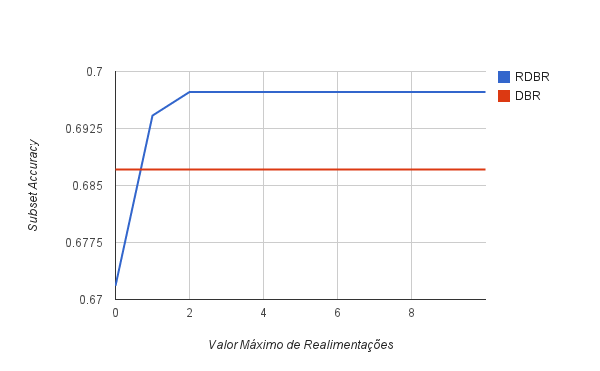
\includegraphics[width=1\textwidth] {Gmedicalj48_mrlm.png}
\end{figure}

\begin{figure}[h]
\label{fig:Gmrlm_2}
\caption{Gráficos do desempenho do \MRLMa~(eixo vertical) para vários valores máximos de iterações (eixo horizontal)
representado nas linha azuis.
A linha em vermelha representa um limiar para o \MRLMa~cujo valor é o desempenho do DBR.}
\centering
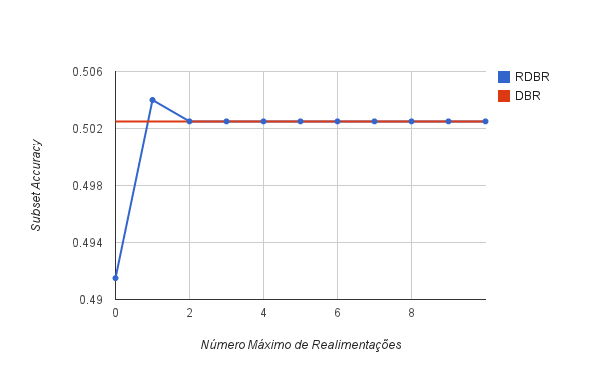
\includegraphics[width=1\textwidth] {Gbirdsj48_mrlm.png}
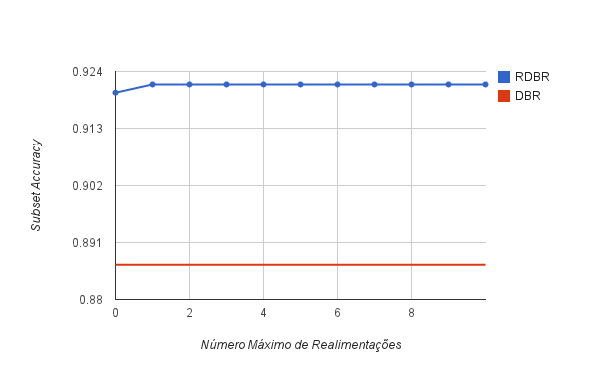
\includegraphics[width=1\textwidth] {Ggenbaseknn_mrlm.png}
\end{figure}



É importante analisar o quanto o método aumenta o tamanho da base de dados uma vez que isso acarreta no aumento
do tempo de execução do algoritmo. Seja $r$ o número de rótulos, $n$ o número de instâncias de treino
e $m$ o número de atributos da base original, na fase de treinamento do \MRLMa, o número de base de dados utilizadas são
$2r$, cada uma contendo $n$ instâncias. Em metade delas, as instâncias contidas tem $m$ atributos e na outra metade $m+r$ atributos.
Já na fase de predição do algoritmo, no pior caso, o algoritmo usa $(r+1)r$ bases de dados de $n$ instâncias onde na primeira base, o
número de atributos é igual a $m$ e nas restantes é igual $m+r$. Vale ressaltar que nem todas essas bases de dados precisam ser
armazenados explicitamente na mémoria em espaços diferentes, algumas podem são reutilizadas no processo de predição.

% Em relação a complexidade algorítma do \MRLMa, ela pode ser
% aproximada pelo número de atributos destinados ao classificador base, uma vez que é um método de transfomação
% e a maior parte do custo computacional se encontra no classificador base.
% A complexidade 




\chapter{Avaliação e Análise Experimental}
Neste capítulo é descrito as bases de dados multirrótulo usadas nos experimentos, as medidas de avaliação escolhidas e a escolha
dos parâmetros dos classificadores. 
A comparação e estudo dos métodos é feita considerando o custo computacional e a qualidade de predição.
A qualidade de predição é estimada pelo método de avaliação por validação cruzada \ref{sec:modelav} com 10 grupos
(\textit{10-fold cross-validation}) sobre \Nbases~bases de dados, todas apresentadas e descritas na subseção \ref{sec:datas}.

Para quantificar a qualidade de predição, 3 métricas foram utilizadas. As métricas escolhidas, bem como o motivo das escolhas,
são listadas:
\begin{itemize}
 \item Subset Accuracy, pois é mostrado que captura bem a correlação entre rótulos;
 \item Hamming Loss, pois é bem mais sensível que o Subset Accuracy;
 \item Example Based Accuracy, é o meio termo entre o Hamming Loss e o Subset Accuracy.
%  \item Tempo computacional, pois é @@@ etc...
\end{itemize}

As fórmulas para o cálculo de cada uma das métricas são apresentadas na seção \ref{sec:metrics}.
É interessante mostrar os resultados experimentais usando diferentes métricas, pois cada uma captura
um aspecto diferente da classificação. 
Num total, foram utilizados \Nml~modelos de classificação multirrótulos: BR, DBR, RDBR, CC, ECC e MCC.
Para cada um deles utilizou-se os seguintes classificadores base: KNN, SVM, J48 e Regressão Logística. 
Para o melhor entendimento, neste capítulo um método multirrótulo é definido como sendo a combinação
de um modelo de classificação multirrótulo com uma configuração de parâmetros pré-definida. Assim, por exemplo,
o classificador BR com KNN é considerado um método diferente do classificador BR com SVM. Isso, por um lado é bom
pois testa o desempenho dos classificadores multirrótulo quando não é gasto tempo computacional para ajustar parâmetros.
Por outro lado é ruim uma vez que considera os mesmos modelos de classificação como sendo completamente diferentes.
Dessa forma, foram considerados 24 métodos multirrótulos e comparados entre si de forma experimental.

\section{Base de dados}
\label{sec:datas}
Todas as 7 bases de dados utilizadas nos experimentos foram obtidas de repositórios públicos pelo seguinte endereço virtual ??.
As bases de dados são apresentadas a seguir:

\begin{itemize}
\item \bf{Emotions}: ??
\item \bf{Scene}: ??
\item \bf{Yeast}: ??
\item \bf{Birds}: ??
\item \bf{Genbase}: ??
\item \bf{Medical}: ??
\item \bf{Enron}: ??	

\end{itemize}
\label{tab:datas}
\begin{table}[h]
\caption{Resumo das bases de dados multirrótulos}
\begin{tabular}{|c|ccccccc|}
\hline
% \textbf{}         & \textbf{}        & \textbf{}         & \multicolumn{2}{c}{\textbf{ATRIBUTOS}} & \textbf{}        & \textbf{}              & \textbf{}          \\
\textbf{BASE}     & \textbf{DOMÍNIO} & \textbf{EXEMPLOS} & \textbf{DIS} & \textbf{NUM} & \textbf{RÓTULOS} & \textbf{CARD} & \textbf{DENS} \\ \hline
\textbf{Emotions} & Música           & 593               & 0                 & 72                 & 6                & 1.869                  & 0.311              \\
\textbf{Scene}    & Imagem           & 2407              & 0                 & 294                & 6                & 1.074                  & 0.179              \\
\textbf{Yeast}    & Biologia         & 2417              & 0                 & 103                & 14               & 4.237                  & 0.303              \\
\textbf{Birds}    & Audio            & 645               & 2                 & 258                & 19               & 1.014                  & 0.053              \\
\textbf{Genbase}  & Biologia         & 662               & 1186              & 0                  & 27               & 1.252                  & 0.046              \\
\textbf{Medical}  & Texto            & 978               & 1449              & 0                  & 45               & 1.245                  & 0.028              \\
\textbf{Enron}    & Texto            & 1702              & 1001              & 0                  & 53               & 3.378                  & 0.064             \\ \hline
\end{tabular}
\end{table}

A tabela \ref{tab:datas} apresenta algumas estatísticas das bases de dados adquiridas.
Nela são apresentadas as seguintes informações de cada base de dados:
\begin{itemize}
  \item \textit{DIS}: número de atributos discretos;
  \item \textit{NUM}: número de atributos numéricos;
  \item \textit{CARD}: cardinalidade de rótulos na base de dados;
  \item \textit{DENS}: densidade de rótulos na base de dados.
\end{itemize}


% \section{Método de Comparação}
% \label{sec:methodcomp}


% 
% Este capítulo se encontra dividido em duas seções, na primeira foram analisados os
% resultados dos métodos de transfomação para cada classificador base.
% Já na segunda seção cada combinação de método multirrótulo com classificador base foi considerado
% um método de transformação e seus resultados são comparados entre si juntamente com os métodos multirrótulos
% de adaptação.


\section{Resultados Experimentais}
Nesta seção é feita uma análise geral do desempenho dos métodos multirrótulos em cada uma das bases de dados
em diferentes métricas.
Para cada métrica escolhida é apresentado uma tabela
contendo os valores das métricas para cada um dos métodos multirrótulo e o
o ranking dos métodos multirrótulos.

% \subsection{Hammin}

\begin{table}[h]
\label{tab:hammingloss}

\caption{EXEMPLO DE TABELA, NAO É DE VERDADE AINDA!}

\end{table}

% \subsection{Medical}
% \subsection{Yeast}
% \subsection{Scene}
% \subsection{Genbase}
% \subsection{Enron}
% \subsection{Birds}

\section{Complexidade Algorítima}




\chapter{Conclusão}